% Template for PLoS

\documentclass[10pt]{article}

% amsmath package, useful for mathematical formulas
\usepackage{amsmath}
% amssymb package, useful for mathematical symbols
\usepackage{amssymb}

% hyperref package, useful for hyperlinks
\usepackage{hyperref}

% graphicx package, useful for including eps and pdf graphics
% include graphics with the command \includegraphics
\usepackage{graphicx}

% Sweave(-like)
\usepackage{fancyvrb}
\DefineVerbatimEnvironment{Sinput}{Verbatim}{fontshape=sl}
\DefineVerbatimEnvironment{Soutput}{Verbatim}{}
\DefineVerbatimEnvironment{Scode}{Verbatim}{fontshape=sl}
\newenvironment{Schunk}{}{}
\DefineVerbatimEnvironment{Code}{Verbatim}{}
\DefineVerbatimEnvironment{CodeInput}{Verbatim}{fontshape=sl}
\DefineVerbatimEnvironment{CodeOutput}{Verbatim}{}
\newenvironment{CodeChunk}{}{}

% cite package, to clean up citations in the main text. Do not remove.
\usepackage{cite}

\usepackage{color}

% Use doublespacing - comment out for single spacing
%\usepackage{setspace}
%\doublespacing


% Text layout
\topmargin 0.0cm
\oddsidemargin 0.5cm
\evensidemargin 0.5cm
\textwidth 16cm
\textheight 21cm

% Bold the 'Figure #' in the caption and separate it with a period
% Captions will be left justified
\usepackage[labelfont=bf,labelsep=period,justification=raggedright]{caption}

% Use the PLoS provided bibtex style
\bibliographystyle{plos}

% Remove brackets from numbering in List of References
\makeatletter
\renewcommand{\@biblabel}[1]{\quad#1.}
\makeatother


% Leave date blank
\date{}

\pagestyle{myheadings}
%% ** EDIT HERE **


%% ** EDIT HERE **
%% PLEASE INCLUDE ALL MACROS BELOW

%% END MACROS SECTION


\begin{document}

% Title must be 150 characters or less
\begin{flushleft}
{\Large
\textbf{Improving access to emergency obstetric care through better referral
systems in rural northern Ghana}
}
% Insert Author names, affiliations and corresponding author email.
\\
  Sneha Patel\textsuperscript{1,2*},
  Christopher B. Boyer\textsuperscript{1},
  J. Koku Awoonor-Williams\textsuperscript{2},
  Rofina Asuru\textsuperscript{2},
  James F. Phillips\textsuperscript{1}\\
\bf{1} Heilbrunn Department of Population and Family Health, Columbia University,  New York,  NY,  USA
\\
\bf{2} Regional Health Administration, Ghana Health Service,  Bolgatanga,  Upper East,  Ghana
\\

\textasteriskcentered{} E-mail:   \href{mailto:sp2827@cumc.columbia.edu}{sp2827@cumc.columbia.edu}
  
  
  
  

\end{flushleft}

\begin{quote}
\textbf{Problem:} Transport and referral system delays block access to
essential emergency obstetric interventions among pregnant women in
rural Ghana. \newline{} \textbf{Approach:} The Sustainable Emergency
Referral Care (SERC) project aims to develop lasting improvements to
emergency transport equipment, communication systems, patient triage
protocols, and financing and supervision of the referral system to
improve access and save lives. \newline{} \textbf{Local Setting:} The
Upper East Region is the epicenter of community-based primary health
care innovation in Ghana and has dramatically improved child survival
despite high rates of poverty. However, geographically-dispersed
populations and a lack of transportation infrastructure are a barrier to
continued improvements in maternal and neonatal health.\newline{}
\textbf{Relevant Changes:} SERC piloted several vehicles Lessons Learnt:
\end{quote}

\section*{Introduction}\label{introduction}
\addcontentsline{toc}{section}{Introduction}

Cite fancy references {[}1{]}.

\section*{Methods}\label{methods}
\addcontentsline{toc}{section}{Methods}

Data for the present study were derived from Ghana's District Health
Information Management System (DHIMS) which records vital health
statistics from all public health facilities in Ghana on a monthly
basis. We consider only tallies of relevant indicators over the period
2009 to 2014, a period that includes a year and a half of data from
fully operational SERC districts. The period prior to 2009 included only

We aim to estimate the impact of SERC services using piecewise spline
regression to model change in mean facility reports of births, maternal
deaths, and cesarian sections in the period before and after the
implementation of SERC. The experience of SERC facilities is compared to
that of a control group comprised of facilities in neighboring districts
in the Upper East and Upper West Regions of Ghana. Controls were
selected with careful consideration

\section*{Results}\label{results}
\addcontentsline{toc}{section}{Results}

\begin{CodeChunk}

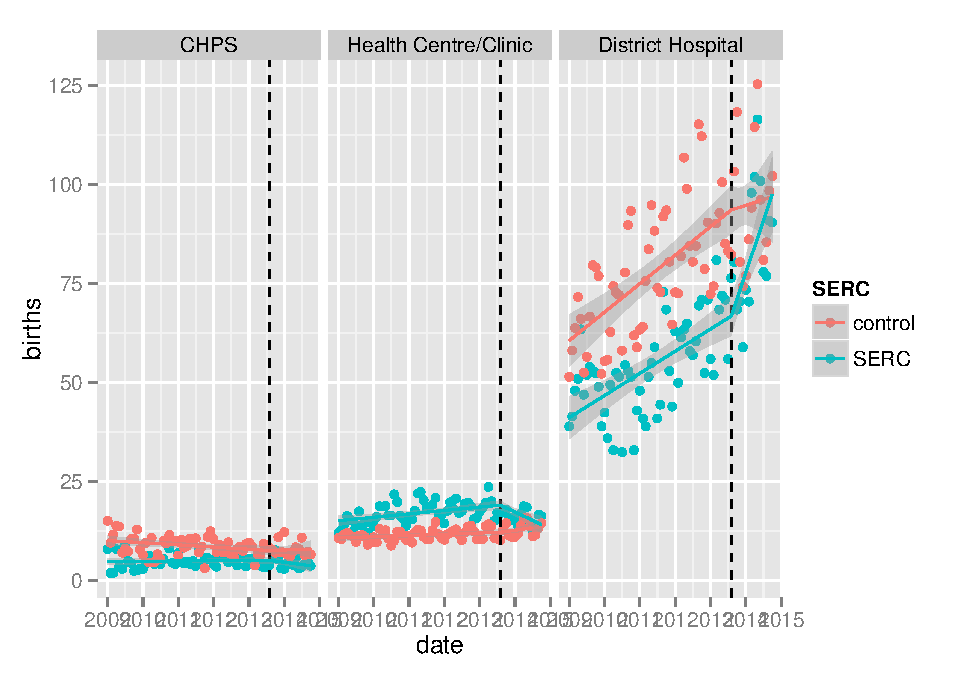
\includegraphics{serc_evaluation_files/figure-latex/unnamed-chunk-2-1} \end{CodeChunk}

\section*{Discussion}\label{discussion}
\addcontentsline{toc}{section}{Discussion}

\section*{Material and Methods}\label{material-and-methods}
\addcontentsline{toc}{section}{Material and Methods}

You may title this section ``Methods'' or ``Models''. ``Models'' is not
a valid title for PLoS ONE authors. However, PLoS ONE authors may use
``Analysis''

\section*{Acknowledgments}\label{acknowledgments}
\addcontentsline{toc}{section}{Acknowledgments}

Do NOT remove this, even if you are not including acknowledgments

\section*{References}\label{references}
\addcontentsline{toc}{section}{References}

A reference list should be automatically created here. However it won't.
Pandoc will place the list of references at the end of the document
instead. There are no convenient solution for now to force Pandoc to do
otherwise. The easiest way to get around this problem is to edit the
LaTeX file created by Pandoc before compiling it again using the
traditional LaTeX commands.

\section*{Figure Legends}\label{figure-legends}
\addcontentsline{toc}{section}{Figure Legends}

\section*{Tables}\label{tables}
\addcontentsline{toc}{section}{Tables}

1. Garnier S, Gautrais J, Theraulaz G (2007) The biological principles
of swarm intelligence. Swarm Intelligence 1: 3--31. Available:
\url{http://www.springerlink.com/index/10.1007/s11721-007-0004-y}.

\end{document}

